\documentclass[10pt,landscape,a4paper]{article}
\usepackage[landscape,margin=0.5in]{geometry}
\usepackage{multicol}
\usepackage{amsmath,amssymb}
\usepackage{graphicx}
\usepackage{xcolor}
\usepackage{tikz}
\usepackage{booktabs}
\usepackage{enumitem}
\usepackage{fancyhdr}
\usepackage{titlesec}

% Compact formatting
\setlength{\parindent}{0pt}
\setlength{\parskip}{2pt}
\setlist[itemize]{leftmargin=*, noitemsep, topsep=0pt}
\setlist[enumerate]{leftmargin=*, noitemsep, topsep=0pt}

% Section formatting
\titleformat{\section}{\normalfont\large\bfseries\color{blue!70!black}}{\thesection}{1em}{}
\titleformat{\subsection}{\normalfont\normalsize\bfseries\color{blue!50!black}}{\thesubsection}{1em}{}
\titlespacing*{\section}{0pt}{6pt}{3pt}
\titlespacing*{\subsection}{0pt}{4pt}{2pt}

% Box for important formulas
\newcommand{\importantbox}[1]{%
  \fcolorbox{blue!50!black}{blue!5}{%
    \parbox{0.92\linewidth}{#1}%
  }%
}

% Highlight color
\newcommand{\highlight}[1]{\colorbox{yellow!30}{$#1$}}

\pagestyle{fancy}
\fancyhf{}
\fancyhead[C]{\textbf{Elementary Metabolic Control Analysis -- V1.0}}
\fancyfoot[C]{\thepage}
\renewcommand{\headrulewidth}{0.4pt}

\begin{document}

\begin{multicols}{3}

% =============================================================================
\section{Core Concept}
% =============================================================================

\subsection{What MCA Quantifies}

MCA asks: if enzyme $E_j$ is perturbed by a small amount, how much does the
steady-state flux $J$ or metabolite concentration $S_i$ change?

\begin{center}
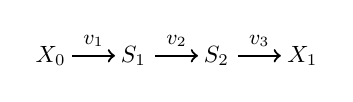
\begin{tikzpicture}[scale=0.78, every node/.style={scale=0.85}]
  \node at (0,0)    {$X_0$};
  \draw[->,thick]   (0.35,0) -- (1.05,0) node[midway,above]{\small $v_1$};
  \node at (1.35,0) {$S_1$};
  \draw[->,thick]   (1.70,0) -- (2.40,0) node[midway,above]{\small $v_2$};
  \node at (2.70,0) {$S_2$};
  \draw[->,thick]   (3.05,0) -- (3.75,0) node[midway,above]{\small $v_3$};
  \node at (4.10,0) {$X_1$};
\end{tikzpicture}
\end{center}

Three types of coefficient capture sensitivity at different scales:

\begin{itemize}
  \item \textbf{Elasticities} $\varepsilon$ --- local, kinetic level
  \item \textbf{Control coefficients} $C$ --- global, system level
  \item \textbf{Response coefficients} $R$ --- combined effect
\end{itemize}

\subsection{Steady State}

At steady state all species concentrations are constant:
\[
  \frac{dS_i}{dt} = 0 \quad \text{for all } i
\]

A unique, stable steady state is assumed throughout.

% =============================================================================
\section{Elasticity Coefficients}
% =============================================================================

Elasticities are \textbf{local} properties of individual rate laws.
They describe how a reaction rate responds to a change in one of its
effectors, holding the enzyme level and all other variables fixed.

\subsection{Scaled Elasticity}

\importantbox{
\[
  \varepsilon_{ij} = \frac{\partial \ln v_i}{\partial \ln S_j}
                  = \frac{S_j}{v_i}\,\frac{\partial v_i}{\partial S_j}
\]
}

\textbf{Interpretation:} a 1\% change in $S_j$ causes an $\varepsilon_{ij}$\%
change in $v_i$.

\subsection{Unscaled Elasticity}

\[
  \varepsilon_{ij}^{u} = \frac{\partial v_i}{\partial S_j}
\]

Used in the Jacobian: $\mathbf{A} = \mathbf{N}\cdot\boldsymbol{\varepsilon}^{u}$.

\subsection{Sign Convention}

\begin{itemize}
  \item $\varepsilon_{ij} > 0$ if $S_j$ \emph{activates} $v_i$ (substrate)
  \item $\varepsilon_{ij} < 0$ if $S_j$ \emph{inhibits} $v_i$ (product, inhibitor)
  \item $\varepsilon_{ij} = 0$ if $v_i$ does not depend on $S_j$
\end{itemize}

\subsection{Common Elasticity Formulas}

\textbf{Michaelis--Menten:} $v = \dfrac{V_{\max}S}{K_m + S}$
\[
  \varepsilon_S = \frac{K_m}{K_m + S} \quad \in (0,\,1)
\]
Near-equilibrium ($S \ll K_m$): $\varepsilon_S \to 1$.
Saturated ($S \gg K_m$): $\varepsilon_S \to 0$.

\textbf{Hill kinetics:} $v = \dfrac{V_{\max}S^n}{K^n + S^n}$
\[
  \varepsilon_S = n\,\frac{K^n}{K^n + S^n} \quad \in (0,\,n)
\]

\textbf{Mass action:} $v = kS$
\[
  \varepsilon_S = 1
\]

\textbf{Competitive inhibition:}
\[
  \varepsilon_I = -\frac{I/K_i}{1 + I/K_i} \quad \in (-1,\,0)
\]

\textbf{Reversible Michaelis--Menten:}
\[
  v = \frac{V_f(S/K_S) - V_r(P/K_P)}{1 + S/K_S + P/K_P}
\]
\[
  \varepsilon_S > 0, \quad \varepsilon_P < 0
\]

\subsection{Haldane Relationship}

For a reversible reaction at equilibrium ($v = 0$):
\[
  \varepsilon_S + \varepsilon_P = 0 \quad \text{and} \quad
  \frac{\varepsilon_S}{\varepsilon_P} = -\frac{v_f}{v_r}
\]

% =============================================================================
\section{Flux Control Coefficients}
% =============================================================================

\subsection{Definition}

\importantbox{
\[
  C_{j}^{J} = \frac{\partial \ln J}{\partial \ln e_j}
            = \frac{e_j}{J}\,\frac{\partial J}{\partial e_j}
\]
}

$C_j^J$ measures the fractional change in steady-state flux $J$
caused by a fractional change in enzyme $e_j$, with all other
enzyme levels held constant.

\subsection{Alternative Form}

Enzyme level $e_j$ is proportional to $V_{\max,j}$, so equivalently:
\[
  C_j^J = \frac{V_{\max,j}}{J}\,\frac{\partial J}{\partial V_{\max,j}}
\]

\subsection{Summation Theorem (Flux)}

\importantbox{
\[
  \sum_{j=1}^{r} C_j^J = 1
\]
}

Control is a shared, conserved resource: if one enzyme gains control,
others must collectively lose the same amount.

\subsection{Properties}

\begin{itemize}
  \item Dimensionless, scaled quantity
  \item Typically $0 \leq C_j^J \leq 1$ for unbranched pathways
  \item Can exceed 1 or be negative at branch points
  \item \textbf{Not} a fixed property of the enzyme -- depends on the
        whole system's operating point
\end{itemize}

\subsection{Intuition}

\begin{itemize}
  \item Fast enzyme (low flux limitation) $\Rightarrow$ low $C_j^J$
  \item Rate-limiting enzyme $\Rightarrow$ $C_j^J \approx 1$
  \item Control is shared; there is rarely a single ``rate-limiting step''
\end{itemize}

% =============================================================================
\section{Concentration Control Coefficients}
% =============================================================================

\subsection{Definition}

\importantbox{
\[
  C_{j}^{S_i} = \frac{\partial \ln S_i}{\partial \ln e_j}
              = \frac{e_j}{S_i}\,\frac{\partial S_i}{\partial e_j}
\]
}

$C_j^{S_i}$ measures how the steady-state concentration of metabolite
$S_i$ changes when enzyme $e_j$ is perturbed.

\subsection{Summation Theorem (Concentration)}

\importantbox{
\[
  \sum_{j=1}^{r} C_j^{S_i} = 0 \quad \text{for all } i
\]
}

Scaling all enzymes by the same factor cannot change any
concentration at steady state (flux rescales but $S_i$ does not).

\subsection{Sign Interpretation}

For an unbranched pathway, increasing an enzyme:
\begin{itemize}
  \item \textbf{Decreases} concentrations of its \emph{upstream} metabolites
        ($C_j^{S_i} < 0$ for $i$ upstream of $j$)
  \item \textbf{Increases} concentrations of its \emph{downstream} metabolites
        ($C_j^{S_i} > 0$ for $i$ downstream of $j$)
\end{itemize}

This is the \textbf{Crossover Theorem}.

%\columnbreak

% =============================================================================
\section{Connectivity Theorems}
% =============================================================================

Connectivity theorems link the global control coefficients to the
local elasticity coefficients.

\subsection{Flux Connectivity}

\importantbox{
\[
  \sum_{j=1}^{r} C_j^J\,\varepsilon_{jk} = 0
  \quad \text{for all metabolites } k
\]
}

\subsection{Concentration Connectivity}

\importantbox{
\[
  \sum_{j=1}^{r} C_j^{S_i}\,\varepsilon_{jk} = -\delta_{ik}
  \quad \text{for all } i, k
\]
}

where $\delta_{ik}$ is the Kronecker delta (1 if $i=k$, else 0).

\subsection{Matrix Form}

Let $\mathbf{C}^J$ be the row vector of flux control coefficients and
$\mathbf{C}^S$ the matrix of concentration control coefficients:

\[
  \mathbf{C}^J \cdot \boldsymbol{\varepsilon} = \mathbf{0}
\]
\[
  \mathbf{C}^S \cdot \boldsymbol{\varepsilon} = -\mathbf{I}
\]

\textbf{Key consequence:} for an $n$-enzyme unbranched chain
(where $\boldsymbol{\varepsilon}$ is square and invertible):
\[
  \mathbf{C}^S = -\boldsymbol{\varepsilon}^{-1}
\]

\subsection{Using the Theorems}

Summation + connectivity theorems provide $n + n$ equations for
the $n$ unknown flux control coefficients of an $n$-enzyme system.
Together they fully determine $\mathbf{C}^J$ from the elasticities alone.

% =============================================================================
\section{Response Coefficients}
% =============================================================================

\subsection{Definition}

A \textbf{response coefficient} describes how a steady-state variable
changes with respect to an \emph{external} parameter $p$ (e.g.\ an
inhibitor concentration, an external substrate level):

\importantbox{
\[
  R_p^J = \frac{\partial \ln J}{\partial \ln p},
  \qquad
  R_p^{S_i} = \frac{\partial \ln S_i}{\partial \ln p}
\]
}

\subsection{Partitioned Response (Chain Rule)}

If parameter $p$ directly affects only reaction $k$:

\[
  R_p^J = C_k^J \cdot \varepsilon_{kp}
\]
\[
  R_p^{S_i} = C_k^{S_i} \cdot \varepsilon_{kp}
\]

\textbf{General case} (parameter affects multiple reactions):
\[
  R_p^J = \sum_k C_k^J\,\varepsilon_{kp}
\]

\subsection{Interpretation}

Response = (system-level control) $\times$ (local sensitivity).
\begin{itemize}
  \item An inhibitor with $\varepsilon_{kp} = -0.8$ applied to an
        enzyme with $C_k^J = 0.3$ gives $R_p^J = -0.24$:
        a 1\% increase in inhibitor reduces flux by 0.24\%.
  \item Even a potent inhibitor ($|\varepsilon|$ large) has little
        effect on flux if $C_k^J$ is small.
\end{itemize}

% =============================================================================
\section{Example: Two-Enzyme Chain}
% =============================================================================

\subsection{System}

\begin{center}
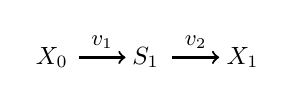
\begin{tikzpicture}[scale=0.85, every node/.style={scale=0.9}]
  \node at (0,0)    {$X_0$};
  \draw[->,thick]   (0.4,0) -- (1.1,0) node[midway,above]{\small $v_1$};
  \node at (1.4,0)  {$S_1$};
  \draw[->,thick]   (1.8,0) -- (2.5,0) node[midway,above]{\small $v_2$};
  \node at (2.85,0) {$X_1$};
\end{tikzpicture}
\end{center}

$X_0, X_1$ fixed externally; one internal species $S_1$.
Elasticities: $\varepsilon_1 \equiv \varepsilon_{1,S_1}$ (product elasticity of $v_1$),
$\varepsilon_2 \equiv \varepsilon_{2,S_1}$ (substrate elasticity of $v_2$).

Typically $\varepsilon_1 < 0$ (product inhibition), $\varepsilon_2 > 0$ (substrate activation).

\subsection{Solving for $C_1^J$ and $C_2^J$}

Summation: $C_1^J + C_2^J = 1$

Flux connectivity ($k = S_1$):
$C_1^J \varepsilon_1 + C_2^J \varepsilon_2 = 0$

\importantbox{
\[
  C_1^J = \frac{\varepsilon_2}{\varepsilon_2 - \varepsilon_1},
  \qquad
  C_2^J = \frac{-\varepsilon_1}{\varepsilon_2 - \varepsilon_1}
\]
}

Since $\varepsilon_2 > 0$ and $\varepsilon_1 < 0$, both coefficients
are positive and sum to 1.

\subsection{Concentration Control}

Summation: $C_1^{S_1} + C_2^{S_1} = 0$

Concentration connectivity:
$C_1^{S_1} \varepsilon_1 + C_2^{S_1} \varepsilon_2 = -1$

\[
  C_1^{S_1} = \frac{1}{\varepsilon_2 - \varepsilon_1} > 0,
  \qquad
  C_2^{S_1} = \frac{-1}{\varepsilon_2 - \varepsilon_1} < 0
\]

Activating $E_1$ (upstream) \emph{raises} $S_1$; activating
$E_2$ (downstream) \emph{lowers} $S_1$.

\subsection{Numeric Example}

Let $\varepsilon_2 = 0.6$, $\varepsilon_1 = -0.4$.
\[
  C_1^J = \frac{0.6}{1.0} = 0.6,
  \quad
  C_2^J = \frac{0.4}{1.0} = 0.4
\]
$E_1$ carries 60\% of flux control; $E_2$ carries 40\%.

% =============================================================================
\section{Example: Three-Enzyme Chain}
% =============================================================================

\subsection{System}

\begin{center}
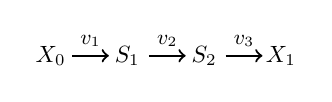
\begin{tikzpicture}[scale=0.78, every node/.style={scale=0.85}]
  \node at (0,0)    {$X_0$};
  \draw[->,thick]   (0.35,0) -- (0.95,0) node[midway,above]{\small $v_1$};
  \node at (1.25,0) {$S_1$};
  \draw[->,thick]   (1.60,0) -- (2.20,0) node[midway,above]{\small $v_2$};
  \node at (2.50,0) {$S_2$};
  \draw[->,thick]   (2.85,0) -- (3.45,0) node[midway,above]{\small $v_3$};
  \node at (3.75,0) {$X_1$};
\end{tikzpicture}
\end{center}

Relevant elasticities ($v_i$ depends on its substrate $S_{i-1}$ and
product $S_i$, with external species fixed):

\begin{align*}
  \varepsilon_{11} &= \frac{\partial \ln v_1}{\partial \ln S_1} < 0
  \quad \text{(product of $v_1$)} \\
  \varepsilon_{21} &= \frac{\partial \ln v_2}{\partial \ln S_1} > 0
  \quad \text{(substrate of $v_2$)} \\
  \varepsilon_{22} &= \frac{\partial \ln v_2}{\partial \ln S_2} < 0
  \quad \text{(product of $v_2$)} \\
  \varepsilon_{32} &= \frac{\partial \ln v_3}{\partial \ln S_2} > 0
  \quad \text{(substrate of $v_3$)}
\end{align*}

\subsection{Connectivity Equations}

For $k = S_1$: \quad $C_1^J \varepsilon_{11} + C_2^J \varepsilon_{21} = 0$

For $k = S_2$: \quad $C_2^J \varepsilon_{22} + C_3^J \varepsilon_{32} = 0$

Together with $\sum C_j^J = 1$, solving gives:

\importantbox{
\begin{align*}
  C_1^J &\propto \frac{\varepsilon_{21}}{\varepsilon_{11}} \cdot
                  \frac{\varepsilon_{32}}{\varepsilon_{22}} \\[4pt]
  C_2^J &\propto \frac{\varepsilon_{32}}{\varepsilon_{22}} \\[4pt]
  C_3^J &\propto 1
\end{align*}
Normalized so that $C_1^J + C_2^J + C_3^J = 1$.
}

\textbf{Adjacent ratio rule:}
\[
  \frac{C_i^J}{C_{i+1}^J} = -\frac{\varepsilon_{i+1,i}}{\varepsilon_{ii}}
\]

% =============================================================================
\section{Example: Branched Pathway}
% =============================================================================

\subsection{System}

\begin{center}
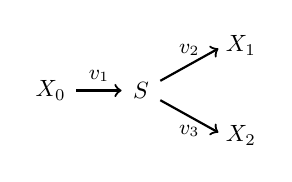
\begin{tikzpicture}[scale=0.82, every node/.style={scale=0.85}]
  \node at (0,0)     {$X_0$};
  \draw[->,thick]    (0.4,0) -- (1.1,0) node[midway,above]{\small $v_1$};
  \node at (1.4,0)   {$S$};
  \draw[->,thick]    (1.7,0.15) -- (2.6,0.65) node[midway,above]{\small $v_2$};
  \draw[->,thick]    (1.7,-0.15) -- (2.6,-0.65) node[midway,below]{\small $v_3$};
  \node at (2.95,0.7)  {$X_1$};
  \node at (2.95,-0.7) {$X_2$};
\end{tikzpicture}
\end{center}

Define flux fractions: $\alpha = v_2/v_1$, $\beta = v_3/v_1$,
with $\alpha + \beta = 1$ at steady state.

\subsection{Branch-Point Effect}

At a branch point, control coefficients can \textbf{exceed~1}:
\[
  C_1^{J_2} = \frac{1}{1 - \alpha\,(\varepsilon_{2S}/\varepsilon_{3S})}
\]

\textbf{Key result:} Only enzymes \emph{in or downstream} of a branch
can control the flux ratio $J_2/J_3$.

Summation still holds separately for each flux:
$\sum_j C_j^{J_2} = 1$ and $\sum_j C_j^{J_3} = 1$.

% =============================================================================
\section{The Jacobian Connection}
% =============================================================================

The unscaled elasticities link MCA to linear stability analysis.

\[
  \mathbf{A} = \mathbf{N} \cdot \boldsymbol{\varepsilon}^{u}
\]

\begin{itemize}
  \item Eigenvalues of $\mathbf{A}$ determine stability
  \item Time constants: $\tau_i = -1/\text{Re}(\lambda_i)$
  \item Control coefficients relate to the DC gain:
        $\mathbf{C}^S \propto \mathbf{G}(0) = -\mathbf{A}^{-1}\mathbf{B}$
\end{itemize}

The \textbf{scaled} elasticities used in connectivity theorems are
related to the unscaled ones by:
\[
  \varepsilon_{ij} = \varepsilon_{ij}^{u}\,\frac{S_j}{v_i}
\]

% =============================================================================
\section{Summary Table}
% =============================================================================

\begin{center}
\footnotesize
\begin{tabular}{@{}p{2.1cm}p{2.2cm}p{2.5cm}@{}}
\toprule
\textbf{Coefficient} & \textbf{Formula} & \textbf{Theorem} \\
\midrule
Elasticity $\varepsilon_{ij}$
  & $\dfrac{\partial\ln v_i}{\partial\ln S_j}$
  & Local; no system theorem \\[8pt]
Flux control $C_j^J$
  & $\dfrac{\partial\ln J}{\partial\ln e_j}$
  & $\sum C_j^J = 1$ \\[8pt]
Conc.\ control $C_j^{S_i}$
  & $\dfrac{\partial\ln S_i}{\partial\ln e_j}$
  & $\sum C_j^{S_i} = 0$ \\[8pt]
Response $R_p^J$
  & $\sum_k C_k^J\,\varepsilon_{kp}$
  & Chain rule \\
\bottomrule
\end{tabular}
\end{center}

\vspace{4pt}
\textbf{Key relationships:}
\begin{enumerate}
  \item Summation + Connectivity $\Rightarrow$ solve for $C$ from $\varepsilon$
  \item $\mathbf{C}^S \cdot \boldsymbol{\varepsilon} = -\mathbf{I}$ (unbranched)
  \item $R_p = C \cdot \varepsilon_{p}$ (partitioned response)
  \item Control can exceed 1 at branch points
\end{enumerate}

\vfill
\hrule
\vspace{3pt}
\footnotesize
\textit{Created by Herbert M. Sauro, \today, Based on: Heinrich \& Schuster (1996); H.M. Sauro, ``Systems Biology: An Introduction to Metabolic Control Analysis; Fell, \textit{Understanding the Control of Metabolism} (1997)}

\end{multicols}
\end{document}
